\subsection{x86}

\myindex{x86!\Instructions!LOOP}
Для организации циклов в архитектуре x86 есть старая инструкция \LOOP. 
Она проверяет значение регистра \ECX и если оно не 0, делает \glslink{decrement}{декремент} \ECX 
и переход по метке, указанной в операнде. 
Возможно, эта инструкция не слишком удобная, потому что уже почти не бывает современных компиляторов, 
которые использовали бы её. Так что если вы видите где-то \LOOP, то с большой вероятностью это 
вручную написанный код на ассемблере.

Обычно, циклы на \CCpp создаются при помощи \TT{for()}, \TT{while()}, \TT{do/while()}.
Начнем с \TT{for()}.
\myindex{\CLanguageElements!for}
Это выражение описывает инициализацию, условие, операцию после каждой итерации
(\glslink{increment}{инкремент}/\glslink{decrement}{декремент}) и тело цикла.

\lstinputlisting{patterns/09_loops/simple/loops_1_RU.c}

Примерно так же, генерируемый код и будет состоять из этих четырех частей.
Возьмем пример:

\lstinputlisting[label=loops_src]{patterns/09_loops/simple/loops_2.c}

Имеем в итоге (MSVC 2010):

\lstinputlisting[caption=MSVC 2010]{patterns/09_loops/simple/1_MSVC_RU.asm}

В принципе, ничего необычного.

GCC 4.4.1 выдает примерно такой же код, с небольшой разницей:

\lstinputlisting[caption=GCC 4.4.1]{patterns/09_loops/simple/1_GCC_RU.asm}

Интересно становится, если скомпилируем этот же код при помощи MSVC 2010 с включенной оптимизацией (\TT{\Ox}):

\lstinputlisting[caption=\Optimizing MSVC]{patterns/09_loops/simple/1_MSVC_Ox.asm}

Здесь происходит следующее: переменную $i$ компилятор не выделяет в локальном стеке, 
а выделяет целый регистр под нее: \ESI. 
Это возможно для маленьких функций, где мало локальных переменных.

В принципе, всё то же самое, только теперь одна важная особенность: 
\ttf не должна менять значение \ESI. 
Наш компилятор уверен в этом, а если бы и была необходимость использовать регистр \ESI в функции \ttf, 
то её значение сохранялось бы в стеке. Примерно так же как и в нашем листинге: 
обратите внимание на \TT{PUSH ESI/POP ESI} в начале и конце функции.

Попробуем GCC 4.4.1 с максимальной оптимизацией (\Othree):

\lstinputlisting[caption=\Optimizing GCC 4.4.1]{patterns/09_loops/simple/1_GCC_O3.asm}

\myindex{Loop unwinding}
Однако GCC просто \IT{развернул} цикл\footnote{\gls{loop unwinding} в англоязычной литературе}.

Делается это в тех случаях, когда итераций не слишком много (как в нашем примере)
и можно немного сэкономить время, убрав все инструкции, обеспечивающие цикл. 
В качестве обратной стороны медали, размер кода увеличился.

Использовать большие развернутые циклы в наше время не рекомендуется, потому что большие
функции требуют больше кэш-памяти%
\footnote{Очень хорошая статья об этом: \DrepperMemory.
А также о рекомендациях о развернутых циклах от Intel можно прочитать здесь: 
[\IntelOptimization 3.4.1.7].}.

Увеличим максимальное значение $i$ в цикле до 100 и попробуем снова. GCC выдает:

\lstinputlisting[caption=GCC]{patterns/09_loops/simple/2_GCC_RU.asm}

Это уже похоже на то, что сделал MSVC 2010 в режиме оптимизации (\TT{\Ox}).
За исключением того, что под переменную $i$ будет выделен регистр \EBX.

GCC уверен, что этот регистр не будет 
модифицироваться внутри \ttf, а если вдруг это и придётся там сделать, то его значение будет сохранено 
в начале функции, прямо как в \main.

\clearpage
\subsection{x86: \olly}
\myindex{\olly}

Скомпилируем наш пример в MSVC 2010 с \Ox и \Obzero и загрузим в \olly.

Оказывается, \olly может обнаруживать простые циклы и показывать их в квадратных скобках, 
для удобства:

\begin{figure}[H]
\centering
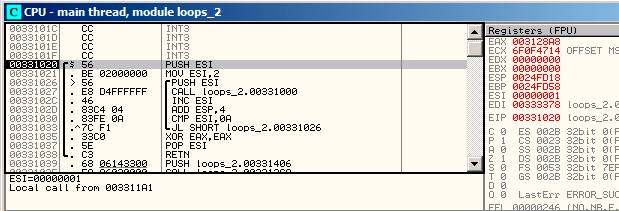
\includegraphics[scale=\FigScale]{patterns/09_loops/simple/olly1.png}
\caption{\olly: начало \main}
\label{fig:loops_olly_1}
\end{figure}

Трассируя (F8~--- \stepover) мы видим, как \ESI увеличивается на 1.

Например, здесь $ESI=i=6$:

\begin{figure}[H]
\centering
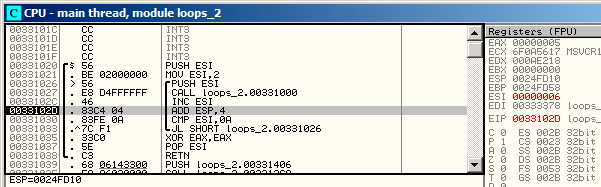
\includegraphics[scale=\FigScale]{patterns/09_loops/simple/olly2.png}
\caption{\olly: тело цикла только что отработало с $i=6$}
\label{fig:loops_olly_2}
\end{figure}

9 это последнее значение цикла.
Поэтому \JL после \glslink{increment}{инкремента} не срабатывает и функция заканчивается:

\begin{figure}[H]
\centering
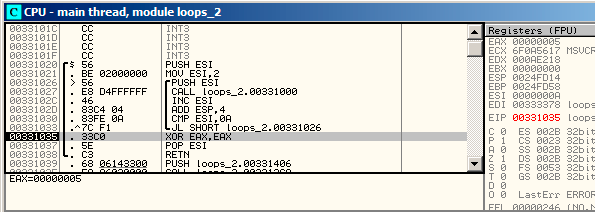
\includegraphics[scale=\FigScale]{patterns/09_loops/simple/olly3.png}
\caption{\olly: $ESI=10$, конец цикла}
\label{fig:loops_olly_3}
\end{figure}

\subsection{x86: tracer}
\myindex{tracer}

Как видно, трассировать вручную цикл в отладчике\EMDASH{}это не очень удобно.
Поэтому попробуем \tracer.
Открываем скомпилированный пример в \IDA, находим там адрес инструкции \INS{PUSH ESI}
(передающей единственный аргумент в \ttf,)
а это \TT{0x401026} в нашем случае и запускаем \tracer:

\begin{lstlisting}
tracer.exe -l:loops_2.exe bpx=loops_2.exe!0x00401026
\end{lstlisting}

Опция \TT{BPX} просто ставит точку останова по адресу и затем tracer будет выдавать состояние регистров.
В \TT{tracer.log} после запуска я вижу следующее:

\lstinputlisting{patterns/09_loops/simple/tracer.log}

Видно, как значение \ESI последовательно изменяется от 2 до 9.
И даже более того, в \tracer можно собирать значения регистров по всем адресам внутри функции.

Там это называется \IT{trace}.
Каждая инструкция трассируется, значения самых интересных регистров запоминаются.
Затем генерируется .idc-скрипт для \IDA, который добавляет комментарии.
Итак, в \IDA я узнал что адрес \main это \TT{0x00401020} и запускаю:

\begin{lstlisting}
tracer.exe -l:loops_2.exe bpf=loops_2.exe!0x00401020,trace:cc
\end{lstlisting}

\TT{BPF} означает установить точку останова на функции.

Получаю в итоге скрипты \TT{loops\_2.exe.idc} и \TT{loops\_2.exe\_clear.idc}.

\clearpage
Загружаю \TT{loops\_2.exe.idc} в \IDA и увижу следующее:

\begin{figure}[H]
\centering
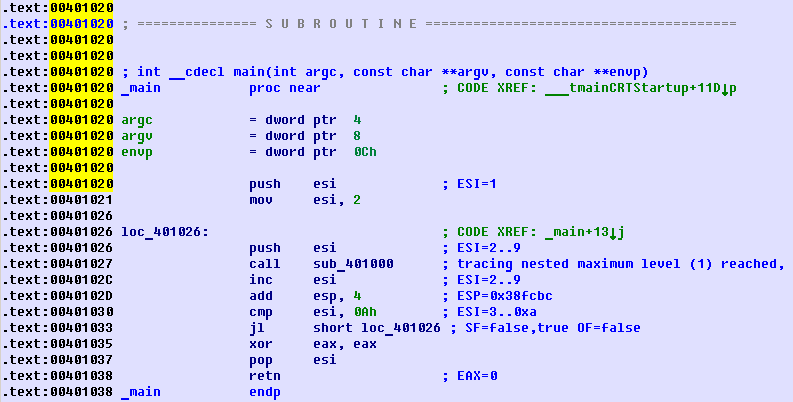
\includegraphics[scale=\FigScale]{patterns/09_loops/simple/IDA_tracer_cc.png}
\caption{\IDA с загруженным .idc-скриптом}
\label{fig:loops_IDA_tracer}
\end{figure}

Видно, что \ESI меняется от 2 до 9 в начале тела цикла, но после 
\glslink{increment}{инкремента} он в пределах [3..0xA].
Видно также, что функция \main заканчивается с 0 в \EAX.

\tracer также генерирует \TT{loops\_2.exe.txt}, 
содержащий адреса инструкций, сколько раз была исполнена
каждая и значения регистров:

\lstinputlisting[caption=loops\_2.exe.txt]{patterns/09_loops/simple/loops_2.exe.txt}
\myindex{\GrepUsage}
Так можно использовать grep.
